% Double-blind submission — WebMedia 2026
\documentclass[sigconf,review]{webmedia}

\usepackage{graphicx}
\usepackage{booktabs}
\usepackage{multirow}
\usepackage{xcolor}
\usepackage{listings}
\lstset{
  basicstyle=\ttfamily\scriptsize,
  frame=single, breaklines=true,
  columns=fullflexible, keepspaces=true
}

\setevent{webmedia}
\proceedingsDetails[WebMedia'2026]{Brazilian Symposium on
  Multimedia and the Web}{2026}{Lavras/MG, Brazil}
\ISSN{2966-2753}

\sloppy

\title{Towards an Automated Accessibility Evaluation Pipeline for
       LLM-Generated Android Jetpack Compose Interfaces}

\author{Leonardo Quezado}
\affiliation{%
  \institution{Universidade Federal do Ceará}
  \city{Fortaleza}
  \country{Brazil}
}
\email{leonardoquezado@proton.me}

\author{Windson Viana}
\affiliation{%
  \institution{Universidade Federal do Ceará}
  \city{Fortaleza}
  \country{Brazil}
}
\email{windson@virtual.ufc.br}

\author{Ribamar de Souza Martins}
\affiliation{%
  \institution{Universidade Federal do Ceará}
  \city{Fortaleza}
  \country{Brazil}
}
\email{ribamarop@gmail.com}

\renewcommand{\shortauthors}{Quezado et al.}

\keywords{LLM, Jetpack Compose, Accessibility, Android, Accessibility Test Framework, Pipeline}

\begin{document}

\begin{abstract}
Research evaluating the quality of artifacts generated by large language
models (LLMs), including code, user interfaces, and media, has expanded
considerably. However, most evaluation remains manual and time-consuming,
making it difficult to keep pace with rapidly released model versions. Recent
work also suggests that newer models can regress relative to their predecessors,
reinforcing the need for continuous and repeatable evaluation. Within this
broader challenge, assessing the accessibility of LLM-generated mobile
interfaces is particularly relevant. This paper presents an end-to-end
automated pipeline for Android Jetpack Compose interfaces, integrating code
extraction, deterministic repair rules, Android compilation, custom Lint
checks, and dynamic Accessibility Test Framework (ATF) execution with minimal
human intervention. We evaluated the pipeline with three LLMs (Claude
Sonnet~4.6, ChatGPT~5.5, and Gemini~3.1 Pro) across eight representative
mobile interface types in light and dark modes. Across 48 evaluations, the
pipeline achieved 100\% compilation success and reported 409 accessibility
findings across static and runtime checks (some of which may correspond to
the same underlying defect). These preliminary results show that end-to-end
automation can support feasible, repeatable, and scalable accessibility
assessment of LLM-generated Compose code while substantially reducing the
manual effort required to evaluate rapidly evolving models.
\end{abstract}

\maketitle

\noindent\textbf{Resumo.}\enspace\textit{%
Pesquisas sobre a qualidade de artefatos gerados por grandes modelos de
linguagem (LLMs), incluindo código, interfaces de usuário e mídia, têm crescido
consideravelmente. No entanto, a maior parte das avaliações ainda é manual e
demorada, o que dificulta acompanhar o ritmo acelerado de lançamento de novas
versões dos modelos. Trabalhos recentes também indicam que versões mais novas
podem regredir em relação às anteriores, reforçando a necessidade de uma
avaliação contínua e reprodutível. Nesse contexto mais amplo, avaliar a
acessibilidade de interfaces móveis geradas por LLMs é particularmente
relevante. Este artigo apresenta um pipeline automatizado de ponta a ponta para
interfaces Android Jetpack Compose, integrando extração de código, regras de
correção determinísticas, compilação Android, verificações Lint customizadas e
execução dinâmica do Accessibility Test Framework (ATF) com mínima intervenção
humana. O pipeline foi avaliado com três LLMs (Claude Sonnet~4.6, ChatGPT~5.5
e Gemini~3.1 Pro) em oito tipos representativos de interface móvel, nos
modos claro e escuro. Ao longo de 48 avaliações, o pipeline alcançou 100\%
de sucesso na compilação e reportou 409 ocorrências de acessibilidade
distribuídas entre análise estática e dinâmica (algumas podendo referir-se
ao mesmo defeito subjacente). Esses
resultados preliminares mostram que a automação de ponta a ponta pode
viabilizar uma avaliação de acessibilidade viável, reprodutível e escalável
de código Compose gerado por LLMs, reduzindo substancialmente o esforço
manual necessário para avaliar modelos em rápida evolução.}

\vspace{4pt}

% ================================================================== %
\section{Introdução}
\label{sec:intro}

O uso de LLMs para geração de artefatos digitais, incluindo código,
interfaces de usuário e mídia, tem se expandido consideravelmente. Paralelamente,
cresce o interesse em avaliar a qualidade desses artefatos de forma sistemática.
Estudos mostram que versões mais recentes de LLMs nem sempre superam as
anteriores em tarefas específicas~\cite{chen2023chatgpt}, reforçando a
necessidade de reavaliação contínua. Nesse contexto mais amplo, avaliar a
acessibilidade de interfaces móveis geradas por LLMs constitui um desafio
particularmente relevante.

Dispositivos Android representam mais de 70\% do mercado global de
smartphones~\cite{businessofapps2025}. O Jetpack Compose modernizou o
desenvolvimento Android~\cite{google2024compose}, mas o Android Lint tem
cobertura limitada para verificações semânticas de acessibilidade em
Compose~\cite{google2024composeaccessibility}. LLMs tornaram-se ferramentas
comuns para desenvolvedores~\cite{peng2023copilot} e código gerado por eles
frequentemente contém omissões de acessibilidade~\cite{suh2025human,anonref3},
porém avaliações automatizadas ainda são escassas para Jetpack Compose.

Um obstáculo prático recorrente nesses estudos é o custo de tempo da
avaliação manual: gerar prompts, compilar, instalar o APK em emulador,
executar ferramentas como o Accessibility Scanner e analisar os resultados
introduz múltiplas etapas manuais de difícil repetição~\cite{anonref1}. Com LLMs lançando novas versões em intervalos
de semanas, resultados obtidos manualmente correm o risco de retratar modelos
que já não existem quando o trabalho é concluído.

Este artigo apresenta resultados parciais de uma pesquisa em andamento que
propõe um pipeline automatizado com cinco estágios para eliminar esse gargalo:
geração de código via LLM, extração e auto-correção, compilação via Docker,
análise estática com Lint customizado e análise dinâmica com o
ATF~\cite{google2024atf}. As questões investigadas são: \textbf{RQ1}~qual a
eficácia do pipeline em compilar código Compose sem intervenção manual;
\textbf{RQ2}~quais categorias de problemas são detectadas;
\textbf{RQ3}~quais diferenças emergem entre Claude, ChatGPT e Gemini nos
déficits de acessibilidade; e \textbf{RQ4}~as ocorrências identificadas pelo
pipeline correspondem às detectadas por avaliação manual com TalkBack e
Accessibility Scanner?

% ================================================================== %
\section{Background e Trabalhos Relacionados}
\label{sec:background}

\subsection{Acessibilidade em Jetpack Compose}

O Jetpack Compose expõe uma árvore semântica paralela à hierarquia de views,
preenchida por modificadores como \texttt{semantics\{\}} e
\texttt{contentDescription}. O ATF~\cite{google2024atf} percorre a árvore de
\texttt{AccessibilityNodeInfo} em tempo de execução e é capaz de verificar:
(i)~ausência de texto acessível em elementos interativos
(\textit{SpeakableTextPresentCheck}); (ii)~alvos de toque abaixo de
48$\times$48\,dp (\textit{TouchTargetSizeCheck}); (iii)~contraste insuficiente
de texto e imagem; e (iv)~duplicidade de rótulos descritivos. Neste trabalho,
as verificações ST, TT e CT são aplicadas via ATF em dispositivo físico;
a verificação de contraste (CT) requer captura de tela obtida via
\texttt{UiAutomation.takeScreenshot()}. As verificações TF e IN são
realizadas pelo Lint customizado (Seção~\ref{sec:customlint}).
Estudos epidemiológicos mostram que problemas de acessibilidade persistem em
proporções significativas das aplicações nas
lojas~\cite{ross2020epidemiology,fok2022longitudinal}.

\subsection{LLMs e Geração de Código de UI}

Suh et al.~\cite{suh2025human} mostraram que LLMs apresentam limitações de
acessibilidade especialmente em requisitos semanticamente complexos, como
atributos ARIA, no domínio web; padrão similar foi documentado em React
Native~\cite{anonref3}. Estudos recentes com avaliadores humanos
confirmaram recorrência de problemas de contraste e rótulos ausentes em
interfaces Android nativas geradas por LLMs~\cite{anonref1}.
Análises em larga escala de apps no Play Store confirmam que omissões de
rótulos são o problema de acessibilidade mais frequente~\cite{fok2022longitudinal}.
Trabalho recente~\cite{anonref2} usou RAG para injetar boas práticas
nos prompts, reduzindo correções manuais de 257 para 144 em 120 telas. O
presente trabalho elimina a intervenção manual por meio de correções
automáticas e utiliza o ATF como avaliador dinâmico, complementando estudos
anteriores com uma perspectiva de análise totalmente automatizada.

% ================================================================== %
\section{Pipeline de Avaliação}
\label{sec:pipeline}

O pipeline, implementado em Python, é composto por cinco estágios ilustrados
na Figura~\ref{fig:pipeline}.

\begin{figure}[h]
\centering
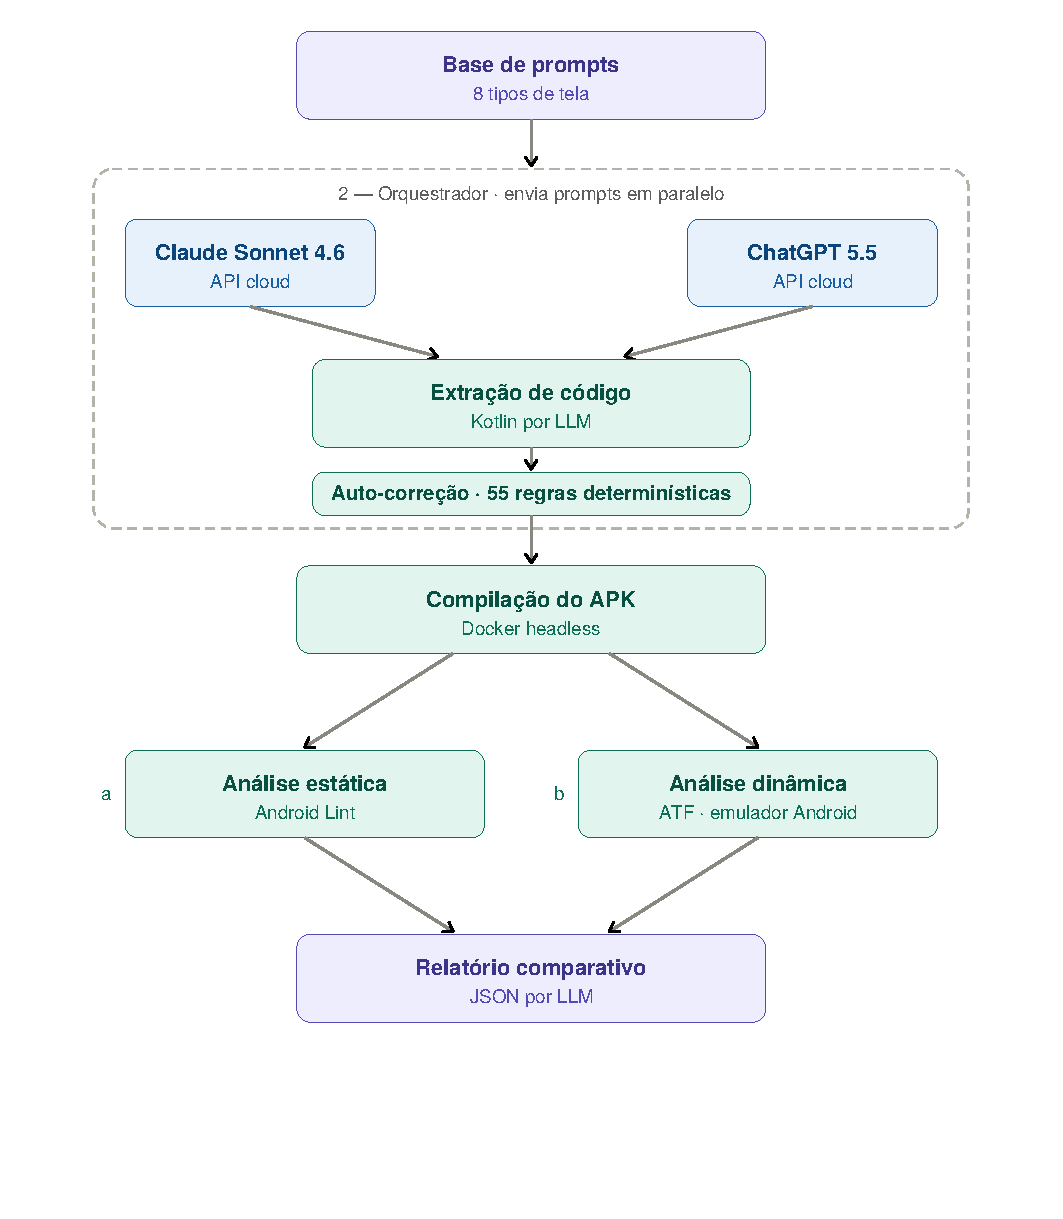
\includegraphics[width=0.95\linewidth, height=5.5cm, keepaspectratio]{pipeline_avaliacao_acessibilidade_v3}
\caption{Estágios do pipeline de avaliação automatizado.}
\label{fig:pipeline}
\end{figure}

\subsection{Design e Template do Prompt}

O prompt é \textit{zero-shot}, sem instruções explícitas de acessibilidade,
para medir o comportamento padrão dos modelos. Cada execução envia dois
blocos ao LLM: (i)~uma \textit{descrição de tela} específica (e.g.,
\textit{``Generate a complete Android E-Commerce screen''}) e (ii)~um
\textit{sufixo fixo} idêntico para todas as execuções, com restrições de
natureza estrutural e de compilação: pacote \texttt{com.accessibility.test},
Jetpack Compose com Material~3, Kotlin, proibição de bibliotecas externas de
imagem (Coil, Glide) e entrega em um único bloco de código. Versões exatas
dos componentes não são fixadas para evitar viés em favor do modelo com treino
mais recente. Nenhuma restrição orienta semanticamente o LLM quanto à
acessibilidade, preservando o caráter \textit{zero-shot} da avaliação.

\subsection{Seleção dos Modelos}

Foram selecionados Claude Sonnet~4.6 (Anthropic), ChatGPT~5.5 (OpenAI) e
Gemini~3.1 Pro (Google), com base em: (i)~desempenho em benchmarks de
geração de código; (ii)~disponibilidade de API; (iii)~ampla adoção entre
desenvolvedores~\cite{peng2023copilot}. Modelos de código aberto foram
excluídos por limitações de infraestrutura, sendo apontados como trabalho futuro.

\subsection{Módulo de Auto-correção}

O módulo foi construído iterativamente: cada falha de compilação motivou a
análise da causa raiz e a adição de uma regra determinística. Exemplo
representativo: os LLMs inseriam \texttt{rememberSaveable} no pacote
incorreto (\texttt{runtime.*} em vez de \texttt{runtime.saveable.*}),
causando \textit{``Unresolved reference''}. Ao todo, 55 regras e 128 testes
de regressão garantem que correções novas não quebrem casos anteriores.
Todas as regras foram finalizadas antes da fase experimental; nenhuma foi
adicionada ou modificada após a observação dos resultados avaliados.
As regras de reparo foram projetadas para corrigir apenas falhas de
compilação. Contudo, sua preservação semântica não foi avaliada de forma
independente.

A Listagem~\ref{lst:violation} ilustra como conformidade sintática não implica
conformidade semântica: o Claude incluiu \texttt{contentDescription\,=\,null},
satisfazendo a assinatura da função mas suprimindo a descrição para
leitores de tela e gerando \textit{ComposeIconNullContentDescription}. Essa
distinção entre presença sintática do parâmetro e seu valor semântico é
central para compreender por que restrições estruturais no prompt não
eliminam violações de acessibilidade.

\begin{lstlisting}[caption={Violação detectada pelo pipeline na tela E-Commerce (Claude~4.6, trecho).},
                   label=lst:violation, language=Kotlin,
                   basicstyle=\ttfamily\tiny]
// Claude 4.6 -- tela E-Commerce (zero-shot, trecho)
IconButton(onClick = { addToCart(product) }) {
    Icon(
        imageVector = Icons.Filled.ShoppingCart,
        contentDescription = null  // ComposeIconNullContentDescription
    )
}
\end{lstlisting}

\subsection{Regras Lint Customizadas}
\label{sec:customlint}

Para contornar a limitação do Android Lint nativo em análise semântica de
Compose, foram desenvolvidas regras customizadas via UAST (\textit{Unified Abstract Syntax Tree}), distribuídas como
módulo Gradle (\texttt{:lint-rules}). As regras detectam em tempo de compilação:
(i)~\texttt{Icon()} com \texttt{contentDescription} ausente ou nulo em
componentes interativos ou como única indicação semântica de uma ação
(\textit{ComposeIconNullContentDescription}); (ii)~\texttt{TextField} e
\texttt{OutlinedTextField} sem parâmetro \texttt{label}, heurística estática
que sinaliza potencial ausência de nome acessível em tempo de execução
(\textit{ComposeTextFieldMissingLabel}). Essa análise estática complementa
a análise dinâmica do ATF, que opera sobre a árvore de acessibilidade em
tempo de execução.

% ================================================================== %
\section{Avaliação Experimental}
\label{sec:avaliacao}

Foram selecionados oito tipos de interface móvel: Login, Configurações,
Dashboard, Chat, Galeria de Fotos, Music Player, E-Commerce e Social Feed.
Cada interface foi gerada pelos três LLMs em dois modos de exibição (claro
e escuro), totalizando 48 execuções. Ambiente de compilação: Ubuntu,
compileSdk/targetSdk~36, Kotlin~1.9.22, AGP~8.2.2, Compose
BOM~2024.02.00, \texttt{espresso-accessibility}~3.5.1, dispositivo físico
(Motorola Edge~60 Fusion, Android~16), mai./2026.\footnote{\url{https://github.com/LeonardoQuezado/accessibility-llm-pipeline}}
O modo escuro foi ativado manualmente via
\texttt{adb shell cmd uimode night yes/no} antes de cada ciclo de
avaliação. Para cada execução: (i)~prompt enviado via API;
(ii)~código submetido ao módulo de auto-correção; (iii)~compilação via
\texttt{./gradlew assembleDebug}; (iv)~execução do Lint customizado e do
ATF (com rolagem: 3 varreduras ascendentes e 3 descendentes); (v)~geração
de relatório JSON. Nenhuma correção manual foi realizada. Os testes ATF
completaram em ~6\,min em média por execução
(mín.\,5,2\,min; máx.\,7,2\,min), totalizando ~4,6\,h de avaliação ATF
nas 48 execuções sem intervenção humana.
Como estudo preliminar, cada configuração (tela $\times$ modelo $\times$
modo) foi avaliada em execução única; a variabilidade estocástica dos LLMs
será controlada em trabalho futuro com múltiplas repetições por
configuração. Ainda assim, os resultados obtidos demonstram que o pipeline
é capaz de detectar as violações para as quais foi projetado, cumprindo o
objetivo central deste artigo curto.

Para validar os resultados do pipeline, três interfaces foram inspecionadas
manualmente com Accessibility Scanner (Google) e TalkBack. O Scanner não
identificou violações estruturais (ST, TF, TT, IN) nas interfaces Music Player
e Login; na interface Social Feed, detectou violações de contraste e rótulos
duplicados. Contraste já é verificado pelo pipeline via \textit{TextContrastCheck}
(CT); rótulos duplicados permanecem fora do escopo atual.
O TalkBack confirmou as deficiências detectadas pelo ATF: botões sem rótulo
foram anunciados sem indicar a ação correspondente, e ícones com
\texttt{contentDescription\,=\,null} foram completamente ignorados pelo leitor
de tela. As divergências entre Scanner e ATF refletem diferenças de cobertura
e modo de execução, não uma hierarquia de rigor entre as ferramentas.

A Tabela~\ref{tab:tempo} compara as ocorrências identificadas pelo pipeline com
as identificadas por avaliação manual (RQ4) nas três interfaces testadas.

\subsection{Validação com Telas Sintéticas}
\label{sec:validacao}

Para verificar o comportamento do pipeline, foram criadas três telas sintéticas
com violações predefinidas (\textit{ground truth}) executadas em dispositivo
físico e emulador. A Tabela~\ref{tab:validation} compara os totais esperados
e obtidos.

\begin{table}[h]
\centering
\caption{Validação com telas sintéticas (LINT e ATF).}
\label{tab:validation}
\setlength{\tabcolsep}{5pt}
{\small
\begin{tabular}{lrrrr}
\toprule
\textbf{Tela}
  & \multicolumn{2}{c}{\textbf{LINT}}
  & \multicolumn{2}{c}{\textbf{ATF (ST)}} \\
\cmidrule(lr){2-3}\cmidrule(lr){4-5}
  & Esp. & Real & Esp. & Real \\
\midrule
ProfileScreen      & 5 & \textbf{5}\,\checkmark & --\textsuperscript{*} & 5\textsuperscript{*} \\
GalleryGridScreen  & 1 & \textbf{1}\,\checkmark & 12 & 16\textsuperscript{†} \\
SettingsFormScreen & 6 & \textbf{6}\,\checkmark &  6 & \textbf{6}\,\checkmark \\
\bottomrule
\multicolumn{5}{l}{\textsuperscript{†}\,4 extras: \texttt{Modifier.size} quebra propagação de} \\
\multicolumn{5}{l}{\texttt{contentDescription} nos \texttt{IconButton}s.} \\
\multicolumn{5}{l}{\textsuperscript{*}\,ATF não predefinido no ground truth; violações detectadas em runtime.} \\
\end{tabular}
}
\end{table}

O LINT correspondeu ao \textit{ground truth} nas três telas. Na
\textit{GalleryGridScreen}, o Lint detectou \textbf{1}~ocorrência de
\texttt{Icon(contentDescription\,=\,null)} no código-fonte, enquanto o ATF
identificou \textbf{16}~instâncias em tempo de execução: 12~itens de grade
e 4~botões cujo \texttt{Modifier.size(28\,dp)} quebrou a propagação de
\texttt{contentDescription}. \textit{TouchTargetSizeCheck} retornou
zero ocorrências pois o \texttt{IconButton} do Material~3 impõe
\texttt{minimumInteractiveComponentSize\,=\,48\,dp} independentemente do
tamanho visual. Na \textit{SettingsFormScreen}, a correlação LINT--ATF foi
perfeita (6--6): cada \texttt{OutlinedTextField} sem \texttt{label} detectado
estaticamente correspondeu a um \texttt{EditText} sem texto acessível no ATF,
confirmando que as duas análises capturam o mesmo problema sob perspectivas
complementares.

\begin{table}[h]
\centering
\caption{Ocorrências detectadas: pipeline vs.\ avaliação manual (Claude Sonnet~4.6).}
\label{tab:tempo}
\setlength{\tabcolsep}{4pt}
{\small
\begin{tabular}{lrrrr}
\toprule
\textbf{Interface} & \textbf{Pipeline} & \textbf{Scanner} & \textbf{TalkBack} & \textbf{Confirm.\textsuperscript{§}} \\
\midrule
Music Player & 6  & 0  & 6                        & \checkmark \\
Login        & 11 & 0  & 3\textsuperscript{†}     & \checkmark \\
Social Feed  & 18 & 8\textsuperscript{‡} & 7{+}   & \checkmark \\
\bottomrule
\multicolumn{5}{l}{Scanner = Accessibility Scanner (Google).} \\
\multicolumn{5}{l}{\textsuperscript{†}\,2 ícones invisíveis ao leitor de tela (IN) + repetição no campo senha (TF).} \\
\multicolumn{5}{l}{\textsuperscript{‡}\,Contraste e rótulos duplicados, tipos distintos dos do pipeline.} \\
\multicolumn{5}{l}{\textsuperscript{§}\,\checkmark indica confirmação qualitativa de ao menos uma categoria} \\
\multicolumn{5}{l}{correspondente; não implica equivalência numérica entre contagens.} \\
\end{tabular}
}
\end{table}

% ================================================================== %
\section{Resultados e Discussão}
\label{sec:resultados}

A Tabela~\ref{tab:results} detalha as ocorrências por tela e modelo.

\begin{table*}[t]
\centering
\caption{Ocorrências por tela (modos claro e escuro combinados).
  ST\,=\,\textit{SpeakableText}; TF\,=\,\textit{TextField} (estático);
  IN\,=\,\textit{IconNull}; TT\,=\,\textit{TouchTarget};
  CT\,=\,\textit{TextContrast}; Tot\,=\,Total.
  Cada linha agrega duas execuções (claro + escuro).}
\label{tab:results}
\setlength{\tabcolsep}{3pt}
{\tiny
\begin{tabular}{l rrrrrr rrrrrr rrrrrr}
\toprule
& \multicolumn{6}{c}{\textbf{Claude Sonnet~4.6}}
& \multicolumn{6}{c}{\textbf{ChatGPT~5.5}}
& \multicolumn{6}{c}{\textbf{Gemini~3.1 Pro}} \\
\cmidrule(lr){2-7}\cmidrule(lr){8-13}\cmidrule(lr){14-19}
\textbf{Tela}
  & ST & TF & IN & TT & CT & Tot
  & ST & TF & IN & TT & CT & Tot
  & ST & TF & IN & TT & CT & Tot \\
\midrule
Login    & 12 &  4 &  0 & 0 &  0 & \textbf{16} & 10 &  4 & 0 & 0 & 0 & \textbf{14} & 10 &  4 & 0 & 0 & 0 & \textbf{14} \\
Config.  &  6 &  4 &  2 & 0 &  0 & \textbf{12} &  6 &  3 & 0 & 0 & 0 & \textbf{ 9} & 10 &  0 & 0 & 0 & 0 & \textbf{10} \\
Dashb.   & 12 &  0 &  4 & 0 &  0 & \textbf{16} &  8 &  0 & 0 & 0 & 0 & \textbf{ 8} &  8 &  0 & 0 & 0 & 0 & \textbf{ 8} \\
Chat     &  8 &  2 &  0 & 0 &  0 & \textbf{10} &  8 &  2 & 0 & 0 & 0 & \textbf{10} &  8 &  2 & 0 & 0 & 2 & \textbf{12} \\
Galeria  & 38 &  2 &  0 & 4 & 12 & \textbf{56} & 38 &  0 & 0 & 4 & 0 & \textbf{42} & 38 &  0 & 0 & 4 & 0 & \textbf{42} \\
Music    & 12 &  0 &  0 & 0 &  2 & \textbf{14} & 12 &  0 & 0 & 0 & 2 & \textbf{14} & 12 &  0 & 0 & 0 & 0 & \textbf{12} \\
E-Com.   &  4 &  0 &  8 & 0 &  2 & \textbf{14} &  8 &  0 & 0 & 0 & 0 & \textbf{ 8} &  8 &  0 & 0 & 0 & 0 & \textbf{ 8} \\
Social   & 14 &  4 &  0 & 0 &  0 & \textbf{18} & 14 &  0 & 0 & 0 & 4 & \textbf{18} & 23 &  0 & 0 & 0 & 1 & \textbf{24} \\
\midrule
\textbf{Total}
  & 106 & 16 & 14 & 4 & 16 & \textbf{156}
  & 104 &  9 &  0 & 4 &  6 & \textbf{123}
  & 117 &  6 &  0 & 4 &  3 & \textbf{130} \\
\bottomrule
\end{tabular}
}
\end{table*}


\subsection{RQ1: Eficácia do pipeline em compilar código gerado}

O pipeline alcançou \textbf{100\%} de sucesso na compilação (48/48 execuções),
sem correções manuais durante as execuções experimentais, resultado direto
do módulo de auto-correção iterativo. O resultado demonstra que a abordagem
determinística de correção é eficaz para normalizar o output dos três LLMs
em ambos os modos de exibição, sem necessidade de prompts mais elaborados
ou modelos fine-tuned para compilação.

\subsection{RQ2: Categorias de problemas detectadas}

O Android Lint nativo reportou \textbf{zero problemas} em todas as 48
execuções, confirmando sua limitação para análise semântica em
Compose~\cite{google2024composeaccessibility}. As regras customizadas
detectaram 31~ocorrências TF e 14~IN (total estático: 45); o ATF
identificou 364~ocorrências dinâmicas (ST=327, TT=12, CT=25), totalizando
\textbf{409~ocorrências}; Lint e ATF podem capturar o mesmo defeito
subjacente por camadas distintas.
\textit{SpeakableTextPresentCheck} (ST) esteve presente em todas as
48~execuções (327~ocorrências), com pico de 38 na Galeria de Fotos
(todos os modelos, em ambos os modos); a menor contagem foi no E-Commerce
do Claude (ST=2 por modo, acompanhado de 4~IN por
\texttt{contentDescription\,=\,null}).
\textit{ComposeTextFieldMissingLabel} (TF) ocorreu nos três modelos:
Claude~16, ChatGPT~9, Gemini~6, com maior concentração no Login e
Configurações.
\textit{TouchTargetSizeCheck} (TT) limitou-se à Galeria de Fotos
(12~ocorrências, 4 por modelo).
\textit{ComposeIconNullContentDescription} (IN) foi exclusivo ao Claude
(14~ocorrências: Configurações~2, Dashboard~4, E-Commerce~8).
\textit{TextContrastCheck} (CT) concentrou-se na Galeria do Claude
(12~ocorrências) e no Social Feed do ChatGPT em modo escuro (4).

\subsection{RQ3: Diferenças entre Claude, ChatGPT e Gemini}

O Claude Sonnet~4.6 registrou o maior número total de ocorrências nos
\textit{outputs} avaliados (\textbf{156}), impulsionado pela exclusividade
de \textit{ComposeIconNullContentDescription} (14~ocorrências: Configurações,
Dashboard e E-Commerce) e pelo maior volume de ocorrências de contraste
(CT=16, concentradas na Galeria). O Gemini~3.1 Pro totalizou \textbf{130},
liderando em \textit{SpeakableText} (ST=117 vs.\ 106 do Claude e 104 do
ChatGPT) e com variação entre modos no Social Feed (10 no claro,
13 no escuro). O ChatGPT~5.5 apresentou o menor total (\textbf{123}), com
distribuição mais homogênea e ausência completa de \textit{IconNull}
(Tabela~\ref{tab:results}).

\textit{SpeakableText} esteve presente em todas as 48~execuções, enquanto
\textit{IconNull} foi exclusivo do Claude. \textit{TextField} foi detectado
nos três modelos: Claude~16, ChatGPT~9 e Gemini~6.
Em síntese, nos \textit{outputs} avaliados, todos os três modelos
produziram interfaces com ocorrências de acessibilidade em ambos os modos,
reforçando a necessidade de avaliação sistemática também em modo escuro.

\subsection{RQ4: Correspondência com avaliação manual}

A Tabela~\ref{tab:tempo} resume os resultados para as três interfaces
testadas com Claude Sonnet~4.6. O TalkBack confirmou 6 ocorrências ST no
Music Player (botões sem rótulo), 3 no Login (ícones invisíveis ao leitor de
tela; campo senha com placeholder duplicado) e 7 no Social Feed (nome,
@usuário, timestamp, imagem e botões de interação sem texto acessível).
O Scanner retornou zero nas duas primeiras interfaces; no Social Feed,
detectou 8 ocorrências de contraste e rótulos duplicados, categorias
complementares não habilitadas na configuração atual do pipeline por
dependerem de captura de tela. A inspeção manual fornece evidência qualitativa de convergência para
categorias selecionadas de ocorrências estruturais reportadas pelo pipeline;
Scanner e ATF revelam categorias complementares.

% ================================================================== %
\section{Conclusão}
\label{sec:conclusao}

Este artigo apresentou um pipeline automatizado de cinco estágios para
avaliar a acessibilidade de interfaces Jetpack Compose geradas por LLMs.
Em 48 avaliações (oito telas, três modelos, modos claro e escuro),
reportou \textbf{409} ocorrências de acessibilidade (estática + dinâmica)
com \textbf{100\%} de compilação bem-sucedida, demonstrando que a validação
automática pode ser integrada ao fluxo de desenvolvimento sem necessidade
de correções manuais durante cada execução. Principais resultados:
(i)~\textit{SpeakableTextPresentCheck} em 48/48 execuções;
(ii)~Claude com maior total (156), incluindo \textit{IconNull} exclusivo (14)
e maior concentração de contraste (CT=16); ChatGPT com menor contagem (123);
Gemini com maior \textit{SpeakableText} (117);
(iii)~déficits observados em ambos os modos de exibição;
(iv)~TalkBack forneceu corroboração qualitativa para categorias selecionadas;
Scanner e ATF revelam categorias complementares.

Ameaças: cada interface foi gerada em execução única (sem controle
estocástico; temperatura~1,0 não garante o mesmo grau de aleatoriedade
entre provedores); o ATF avaliou rolagem básica, mas não navegação entre
telas nem estados condicionais; o modo escuro foi alternado manualmente,
não de forma automatizada; a preservação semântica das regras de reparo
não foi verificada independentemente; os totais são contagens brutas, não
taxas normalizadas. Trabalhos futuros: incluir modelos abertos, explorar
few-shot e RAG, incorporar verificações WCAG adicionais e conduzir estudos
com usuários com deficiência visual.

% ================================================================== %
\smallskip\noindent\textbf{Cuidados Éticos.} Esta pesquisa não recrutou
participantes humanos e utilizou ferramentas automatizadas sobre código
gerado por LLMs. Os autores declaram o uso de Claude Sonnet~4.6 como
apoio à escrita e programação, em conformidade com a Resolução
CNS~n.º~510/2016.

% ================================================================== %
\bibliographystyle{ACM-Reference-Format}
\bibliography{references}

\end{document}
